\documentclass[conference,letterpaper]{IEEEtran}
\usepackage[utf8]{inputenc}
\usepackage[T1]{fontenc}
\usepackage[english]{babel}
\renewcommand{\IEEEkeywordsname}{Index Terms}
\usepackage{cite}
\usepackage{amsmath,amssymb,graphicx,booktabs,tikz}
\usepackage[hidelinks]{hyperref}
\newcommand{\doi}[1]{\href{https://doi.org/#1}{\nolinkurl{#1}}}
\graphicspath{{../figuras/}{figuras/}}
\title{Partial Kinematic Synthesis of a Finger Exoskeleton Mechanism Using Differential Evolution and a Genetic Algorithm}
% The evaluation version defines \versionciega before reading this file.
\ifdefined\versionciega
  \author{}
\else
  \author{
\IEEEauthorblockN{Adriana Elorza-Ramos\IEEEauthorrefmark{2}, Pavel Palma-Nicolás\IEEEauthorrefmark{1},\\
Manuel Arias-Montiel\IEEEauthorrefmark{1} and Esther Lugo-González\IEEEauthorrefmark{1}}
\IEEEauthorblockA{\IEEEauthorrefmark{1}Institute of Electronics and Mechatronics\\
\IEEEauthorrefmark{2}Graduate Studies Division\\
Universidad Tecnológica de la Mixteca, Huajuapan de León, Oaxaca, Mexico\\
\texttt{\{eora010314,panp000112\}@gs.utm.mx}, \texttt{\{mam,elugog\}@mixteco.utm.mx}\\
\footnotesize ORCID: Adriana \href{https://orcid.org/0009-0008-8398-3191}{0009-0008-8398-3191};
Pavel \href{https://orcid.org/0009-0005-9704-9867}{0009-0005-9704-9867}\\
\footnotesize Manuel \href{https://orcid.org/0000-0003-4534-9401}{0000-0003-4534-9401};
Esther \href{https://orcid.org/0000-0002-7374-3425}{0000-0002-7374-3425}}
}
\fi
\begin{document}
\maketitle
\begin{abstract}
This work uses two optimization techniques, Differential Evolution (DE) and the Genetic Algorithm (GA), both implemented in Python, to obtain the partial dimensional synthesis of a finger exoskeleton mechanism aimed at reproducing a precision pinch, fitting the motion up to the middle phalanx and the position of its endpoint, the distal interphalangeal joint (DIP). The problem is formulated with 16 design parameters and an angular-tracking objective function with respect to a 120-sample reference obtained from the database \cite{r1}. Penalties are added to maintain mechanism closure, clearance from the finger, dorsal placement, and adequate height and transmission. The comparison uses the same bounds, 20 seeds, and 4096 evaluations per run. The selected solutions achieve global position errors of 0.298 mm for DE and 0.198 mm for GA. DE produces a more compact mechanism according to the sum of structural lengths: 328.29 mm versus 353.36 mm for GA. GA obtains lower error at both points: 0.169 mm at PIP and 0.222 mm at DIP, versus 0.216 and 0.361 mm for DE. Because of its smaller size, the DE solution is selected to build the assembly in SolidWorks and verify its motion. Its trajectories show errors with respect to the kinematic model of 0.106 mm at PIP and 0.112 mm at DIP. The results show a trade-off between tracking and compactness.
\end{abstract}
\begin{IEEEkeywords}
differential evolution, genetic algorithm, dimensional synthesis, hand exoskeleton, dimensional optimization, mechanism chain.
\end{IEEEkeywords}

\section{Introduction}
Hand exoskeletons are robotic devices for assistance and rehabilitation whose function is to accompany or help restore finger motion \cite{r2}. For assistance to be comfortable and safe, the mechanism must faithfully reproduce the natural joint trajectories of the finger throughout the intended flexion range. Differences between the finger motion and the device can generate unwanted reaction forces at the joints and affect user comfort \cite{r3}. Achieving this tracking depends largely on correctly choosing the lengths of the mechanism links, a problem known as dimensional synthesis \cite{r4}.

Dimensional synthesis for path generation is a difficult optimization problem. The solution space contains broad regions in which the mechanism simply does not assemble or reverses its motion, and the relationship between link lengths and the curve described by the mechanism is nonlinear and has many local optima. Therefore, population-based metaheuristics such as Differential Evolution (DE) and Genetic Algorithms (GAs) are used, as they can explore the search space without requiring derivative information \cite{r4,r5}.

Although both optimization techniques are widely used, which of the two is more effective depends on the nature of the problem, the way the variables are represented, and the tuning of the hyperparameters \cite{r6,r7}. The choice between one or the other is rarely evident and almost always requires testing them on the specific case to be solved.

Dimensional synthesis of linkages for path generation has historically been addressed with analytical methods and, more recently, with metaheuristics, which allow nonconvex functions to be explored without calculating derivatives \cite{r4,r5}. Four-bar mechanisms are a recurrent building block in path synthesis because of their simplicity and their ability to approximate coupler curves with few parameters \cite{r4,r5}. Six-bar chains, such as the Stephenson-II mechanism, have also been studied in finger exoskeletons \cite{r8}. When several four- and five-bar stages are chained, the number of variables grows and different local solutions arise. A change in length affects not only the trajectory of one stage, but also the motion transmitted to the next; therefore, the set of links is studied rather than each stage separately.

In the field of hand exoskeletons, swarm-based optimization has been used to adjust the dimensions of mechanisms that reproduce finger flexion \cite{r8}. Direct comparison between algorithm families has also been studied \cite{r6,r7}. Both DE and a real-coded GA can work with continuous variables. Their results depend on the operators and the chosen parameters, so their behavior must still be studied for the specific mechanism \cite{r9,r10}.

To compare DE and GA, the same objective function, the same design bounds, and the same number of evaluations are maintained \cite{r6,r17}. In addition, the same initial population is used in each pair of runs. Thus, both methods test the same number of designs; matching only the number of generations does not guarantee this condition. The comparison considers tracking error and the sum of lengths to choose a solution suitable for manufacturing.

To make the comparison reproducible, a partial version of the mechanism is optimized, reproducing motion up to the middle phalanx. This case is smaller than the complete three-phalanx model, but retains the essential difficulties of the problem: coupling between stages and assembly and space constraints over the finger. This makes it possible to study the effect of the optimization algorithm without the added complexity of the distal stage. In addition, the mechanism with the dimensions optimized by DE is built in SolidWorks and its trajectories are checked.

\subsection{Contributions}
The contributions of this article are: (i) a formulation of the partial dimensional-synthesis problem with 16 parameters and geometric constraints; (ii) a comparison of DE and GA with the same budget and several seeds, considering error and size; and (iii) a comparison between the kinematic model and the motion study of the optimized mechanism in SolidWorks.

\section{Kinematic model of the exoskeleton}
Fig.~\ref{fig:dedo} shows the initial design; the dimensions resulting from the optimization are presented later. The device reproduces finger flexion through a chain of coupled stages driven by a single input crank $L_1$. The first stage combines a five-bar mechanism ($L_1$, $L_2$, $L_3$, $L_4$, and ground link $B_1$) and a four-bar mechanism ($L_4$, $L_5$, the equivalent support, and ground link $B_2$). The offsets $h_{sp}$ and $d_{sp}$ form a rigid support whose distance between centers is $\sqrt{h_{sp}^2+d_{sp}^2}$. This stage carries motion from the metacarpophalangeal joint (MCP) to the proximal phalanx.

The next stage transmits motion through $L_6$, $L_7$, $L_8$, and arm $c_2$ to the middle body. The proximal $F_p$ and middle $F_m$ phalanges form the finger line, with the MCP, proximal interphalangeal (PIP), and distal interphalangeal (DIP) points, while the linkage chain is placed on the dorsal side. Arm $c_2$ is rigid with respect to the middle phalanx; its relative orientation is defined by auxiliary angle $\theta_{aux}$. MCP and PIP flexion are studied. DIP represents the endpoint of the middle phalanx, not a third actuated flexion.

\begin{figure}[t]
\centering\begingroup
\newdimen\unidadfigura
\unidadfigura=\dimexpr\linewidth/255\relax
\begin{tikzpicture}[x=\unidadfigura,y=\unidadfigura]
\node[anchor=south west,inner sep=0] at (0,0)
 {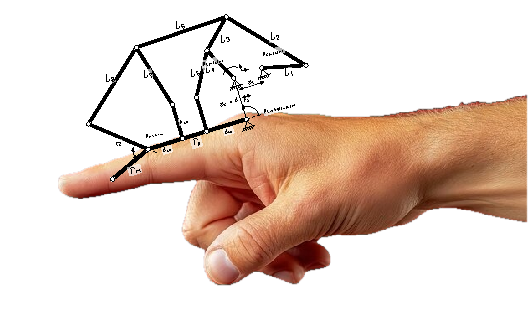
\includegraphics[width=\linewidth]{mecanismo_sobre_dedo_sin_dos_angulos.pdf}};
\end{tikzpicture}
\endgroup

\caption{Simplified finger-mounted exoskeleton mechanism. The geometry of the base design before optimization is retained. $\theta_{1\mathrm{initial}}$ corresponds to $L_4$ and $\theta_{2\mathrm{initial}}$ to $L_1$, with respect to the positive horizontal axis.}
\label{fig:dedo}
\end{figure}

Revolute joints are drawn as circles and fixed supports with hatching. The model stops at the middle phalanx; the distal stage of the complete mechanism is not part of this comparison. The index-finger lengths used are $F_p=46$ mm and $F_m=27$ mm. The distal phalanx measures 22 mm, but it is not involved in the partial study.

The base keeps MCP and the two input pivots fixed. $B_1=18$ mm, $B_2=20$ mm, and a transmission ratio $r_g=2$ are used. Given the orientation $\theta_2$ of $L_1$, that of $L_4$ is obtained from
\begin{equation}
\theta_1=\theta_2/r_g+\theta_{off}.
\end{equation}
Offset $\theta_{off}$ sets its initial relative position. Forward kinematics successively solves the circle intersections imposed by the bar lengths, maintaining the same assembly configuration throughout the motion. This yields the PIP and DIP positions.

\section{Optimization problem formulation}
\subsection{Design variables}
The design vector contains $L_1$--$L_8$, $c_2$, $h_{sp}$, $d_{sp}$, $\theta_{aux}$, the initial orientation and travel of $L_1$, offset $\theta_{off}$, and a fixed rotation of the mechanism with respect to the reference. The ground links, phalanges, and the 2:1 ratio are kept constant. Table~\ref{tab:limites} summarizes the bounds used. The auxiliary angle describes the geometry of the middle body and is not, by itself, a bound on joint flexion.

\begin{table}[t]
\caption{Design variables and search bounds}
\label{tab:limites}\centering\footnotesize
\begin{tabular}{lrr}\toprule Parameter & Min. & Max.\\\midrule
$L_1$ (mm)&29.147&45.147\\ $L_2$ (mm)&31.205&51.205\\
$L_3$ (mm)&12.187&28.187\\ $L_4$ (mm)&14.633&28.633\\
$L_5$ (mm)&9.906&21.906\\ $L_6$ (mm)&51.273&71.273\\
$L_7$ (mm)&18.805&34.805\\ $L_8$ (mm)&38.985&58.985\\
$c_2$ (mm)&29.349&45.349\\ $h_{sp}$ (mm)&18.974&28.974\\
$d_{sp}$ (mm)&4.663&12.663\\ $\theta_{aux}$ (rad)&0.596&1.196\\
Initial angle of $L_1$ (rad)&$-0.545$&0.155\\
Offset $\theta_{off}$ (rad)&1.378&2.078\\
Travel of $L_1$ (rad)&1.663&2.663\\
Mounting rotation (rad)&2.661&3.361\\\bottomrule
\end{tabular}
\end{table}

\subsection{Objective function}
The public database of Jarque-Bou, Atzori, and Müller \cite{r1} contains kinematic records of different hand movements and grasps. For this study, a file of 120 angular samples corresponding to a precision pinch is available. Its angles are converted into positions using the indicated phalanx lengths. For the search, 32 samples distributed along the motion are selected; trajectory errors are then calculated over the 120 samples.

The fitting considers the differences between the joint angles of the mechanism and those of the reference. Each difference is multiplied by the length of the corresponding phalanx and combined with penalties for lack of closure, insufficient clearance from the finger, position outside the dorsal side, excessive height, and unfavorable transmission. If $r_j$ is each component of this set of errors and penalties, the quantity minimized is
\begin{equation}
J=\frac{1}{N_r}\sum_{j=1}^{N_r}r_j^2.
\label{eq:objetivo}
\end{equation}
The components are expressed in mm through their weighting factors, so $J$ is expressed in mm$^2$. This value is used to guide the search; it is not the position error of the trajectories.

The factors used are 1 for the angular error multiplied by length, 30 for closure, 4 for clearance, dorsal position, and height, and 0.5 mm/degree for transmission. The penalties are activated when the corresponding bound is exceeded. The same objective is retained for DE and GA. Sensitivity to angular weighting is reviewed in the discussion.

Table~\ref{tab:restricciones} summarizes the conditions checked when selecting the final solutions. A small penalty does not replace this geometric review. A total of 501 positions are evaluated per solution, and the check is repeated with 5001 positions for the selected designs.

\begin{table}[t]
\caption{Geometric constraints of the partial model}
\label{tab:restricciones}\centering\footnotesize
\begin{tabular}{p{.37\columnwidth}p{.52\columnwidth}}\toprule
Condition & Check\\\midrule
Closure of the four loops & Maximum defect $\leq10^{-7}$ mm\\
Support geometry & $F_p>2d_{sp}$; positive dimensions\\
Finger clearance & Estimated clearance $\geq1$ mm\\
Dorsal location & Signed dorsal distance $\geq1$ mm\\
Height over the finger & Planar estimate $<55$ mm\\
Transmission & Minimum angle $\geq25^\circ$\\\bottomrule
\end{tabular}
\end{table}

To estimate clearance and height, 17 points on each bar are checked. In the motion plane, the finger is represented by a 6-mm-wide strip on each side of its axis, and a 3-mm margin is reserved for the bar. These are geometric approximations used equally in both optimizations, not measurements of the CAD thickness. The current assembly uses links 4 mm thick; interference between solids and screws must be checked in the three-dimensional model.

\section{Evaluation of the optimization techniques}
Both algorithms are run with 20 seeds, from 0 to 19, and 4096 objective-function evaluations per run. Each evaluation corresponds to testing a complete design vector. A population of 64 individuals, included in that budget, is used. For each seed, the initial population and the initial design are shared; the solution from seed 12 is not introduced as an initial point.

The variation parameters selected through Optuna \cite{r13} are the range of the DE mutation factor and recombination probability, and the crossover and mutation probabilities and their distribution indices for GA. In the compared runs, they are kept fixed at the values indicated below. No local tuning or early stopping is used, to respect the same budget in both methods. The code is run in Python with NumPy; SciPy is used in the statistical analysis. Means and standard deviations are calculated over the 20 runs, including those whose best solution does not satisfy all the conditions in Table~\ref{tab:restricciones}.

\subsection{Differential Evolution}
Differential Evolution is a population-based technique for optimization in continuous spaces, whose variants and applications are described in \cite{r14,r15}. The \texttt{best1bin} strategy is implemented: each trial vector starts from the best individual and the scaled difference between two others. The mutation factor $F$ is drawn from a uniform distribution between 0.54 and 0.85 once per generation; it controls how much that difference influences the result. The recombination probability $CR=0.77$ determines which components of the trial vector are inherited from mutation, forcing at least one. Selection retains the trial vector if its objective does not worsen that of the replaced individual. The population is updated once the candidates of the generation have been evaluated.

The range of $F$ controls the sizes of the changes that are tested, and $CR$ governs the combination of new components with those of the individual being modified. These are algorithm parameters, not mechanism dimensions.

Differential mutation adapts the size of changes to population dispersion. When individuals are separated, the changes can be larger; when they concentrate, the changes tend to decrease. This describes the operator, but does not guarantee that it will always find the best solution.

\subsection{Genetic Algorithm}
A real-coded GA is implemented with tournament selection of size 3, simulated binary crossover (SBX) \cite{r16}, and polynomial mutation. The crossover probability per pair is 0.63, with selection of each component with probability 0.5. Mutation is applied per variable with probability 0.22. The distribution indices are 16 for SBX and 14 for mutation. In complete generations, two elite individuals are retained and their evaluations are reused. In the last generation, only two offspring are generated to complete the budget, and the other 62 individuals are retained.

The tournament favors individuals with lower objective values, crossover combines values from two parents, and mutation introduces additional variations. The distribution indices control how close the new values usually remain to the previous ones; the two elite individuals retain the best solutions. The probability 0.5 per component is a crossover rule, whereas the probabilities 0.63 and 0.22 and the indices 16 and 14 define its configuration. The population has 64 individuals in both methods.

\section{Results}
\subsection{Fitting error}
Table~\ref{tab:resultados} brings together the results of both methods and the errors of their selected solutions. For each algorithm, the run with the lowest $J$ that satisfies the constraints is selected: seed 12 for DE and seed 7 for GA. The global position error is calculated as the square root of the mean squared distances of the two PIP and DIP points with respect to the target.

\begin{table}[t]
\caption{Comparison of DE and GA with an equivalent budget}
\label{tab:resultados}\centering\footnotesize
\begin{tabular}{lrr}\toprule Metric & DE & GA\\\midrule
Runs &20&20\\ Evaluations per run &4096&4096\\
Mean $J$ (mm$^2$)&0.001484&0.001504\\
Standard deviation (mm$^2$)&0.001069&0.001192\\
Solutions satisfying constraints&14/20&11/20\\\midrule
Selected seed&12&7\\
Selected $J$ (mm$^2$)&0.000419&0.000242\\
Global RMSE error (mm)&0.2976&0.1976\\
PIP RMSE (mm)&0.2162&0.1693\\
DIP RMSE (mm)&0.3611&0.2223\\
Maximum estimated height (mm)&51.016&54.376\\\bottomrule
\end{tabular}
\end{table}

GA obtains the lowest global error and the lowest error at both points for these solutions. On the other hand, DE has a slightly lower mean $J$ and more solutions satisfying the constraints. The Wilcoxon signed-rank test \cite{rwilcoxon}, which compares the differences between pairs without requiring normality, is applied; its interpretation assumes symmetry in the distribution of those differences. Each pair corresponds to the same seed and initial population. The two-sided test on the 20 differences in $J$ does not detect a significant difference ($W=105$, $p=1.000$, level 0.05). This does not demonstrate equivalence or general superiority of either algorithm.

\begin{figure*}[t]
\centering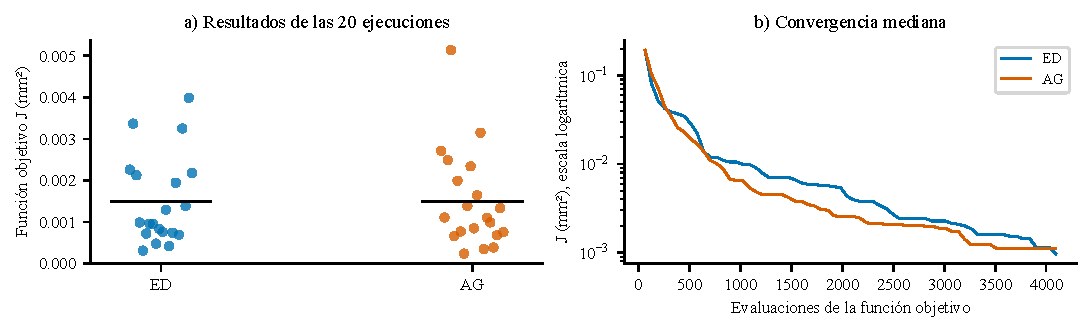
\includegraphics[width=\textwidth]{comparacion_semilla12.pdf}
\caption{Comparison between DE and GA: (a) each point represents the best objective of one run and the black line indicates the mean; (b) median convergence of the 20 runs versus the number of evaluations.}
\label{fig:convergencia}
\end{figure*}

\subsection{Dimensional analysis}
Table~\ref{tab:dimensiones} compares, link by link, the dimensions of the base CAD design with those optimized by DE and GA. The sum of $B_1$, $B_2$, $L_1$--$L_8$, and $c_2$ is 328.29 mm for DE, 353.36 mm for GA, and 380.01 mm for the base design. The DE solution has a sum 7.09\% lower than GA and an estimated planar height of 51.02 mm, versus 54.38 mm. This favors its selection when reducing size over the hand is desired.

Compactness is desirable for manufacturing and device portability. However, the sum of lengths is not equivalent to assembly weight or volume. A reduction in mass will also depend on cross sections, materials, supports, and fasteners.

\begin{table}[t]
\caption{Link dimensions (mm): base CAD design and selected DE and GA solutions}
\label{tab:dimensiones}\centering\footnotesize\begin{tabular}{lrrr}\toprule Parameter & Base CAD & DE & GA\\\midrule
$B_1$ & 18.00 & 18.00 & 18.00\\
$B_2$ & 20.00 & 20.00 & 20.00\\
$L_1$ & 35.00 & 30.33 & 39.56\\
$L_2$ & 49.00 & 40.17 & 42.40\\
$L_3$ & 25.00 & 21.01 & 27.52\\
$L_4$ & 20.00 & 16.55 & 15.57\\
$L_5$ & 25.00 & 13.72 & 14.82\\
$L_6$ & 55.00 & 55.99 & 64.25\\
$L_7$ & 35.00 & 29.13 & 31.49\\
$L_8$ & 52.00 & 46.90 & 40.74\\
$c_2$ & 46.01 & 36.50 & 39.02\\
$h_{sp}$ & 17.00 & 23.71 & 21.83\\
$d_{sp}$ & 18.00 & 7.28 & 7.62\\
\midrule $\sum L_{est}$ & 380.01 & 328.29 & 353.36\\\bottomrule
\end{tabular}
\end{table}

\subsection{Trajectory tracking}
Fig.~\ref{fig:trayectorias} shows the trajectories calculated by DE and GA together with the angular reference used. Both reproduce the general shape of the motion. The global errors are 0.298 and 0.198 mm, respectively. The difference in fit favors GA, whereas the size of the solution favors DE.

Tracking is evaluated at corresponding positions along the motion, without a free alignment that reduces the error. Chamfer distance \cite{r11} and Procrustes fitting \cite{r12} make it possible to study shape similarity, but they are not the metrics used in this comparison. Here, the relationship between crank input and phalanx motion is retained.

\begin{figure*}[t]
\centering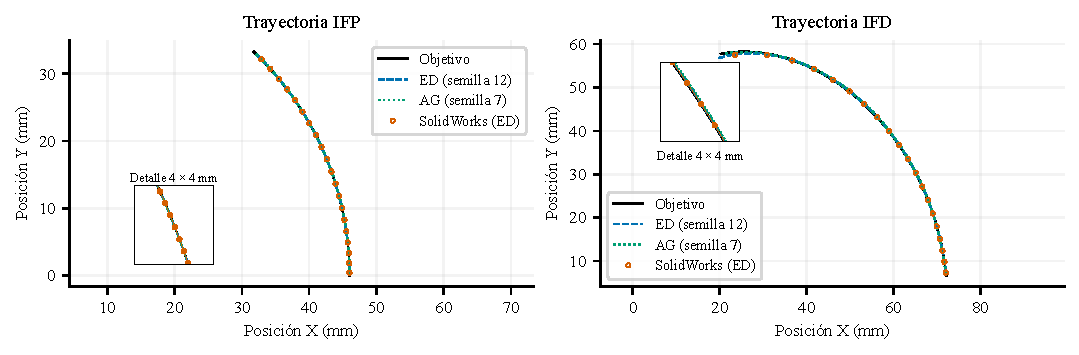
\includegraphics[width=\textwidth]{trayectorias_semilla12.pdf}
\caption{Target trajectories, DE and GA trajectories, and SolidWorks paths of the DE design from seed 12. The $4\times4$ mm details show the differences without shifting the curves.}
\label{fig:trayectorias}
\end{figure*}

\subsection{Convergence}
Fig.~\ref{fig:convergencia} shows the decrease in the objective during the search. The horizontal axis represents evaluations, not generations, to compare the same computational effort. Dispersion among runs of both methods is observed. The budget makes it possible to obtain useful solutions, but does not demonstrate that the global minimum has been found.

\subsection{Simulation of the optimized mechanism}
The assembly from seed 12 is built in SolidWorks with 46- and 27-mm phalanges (Fig.~\ref{fig:cad}). A total of 60 positions of the endpoint of $L_1$, PIP, and DIP are exported at the same instants. The input angle is obtained from the endpoint of $L_1$ and its fixed pivot; the kinematic model is evaluated at those same input positions.

The study spans 141.000$^\circ$, compared with the 139.295$^\circ$ of the optimized solution. The 60 samples are retained to compare SolidWorks with the model. The last one is outside the reference interval and is not used in the comparison with the objective, which contains 59 common positions.

\begin{figure}[t]
\centering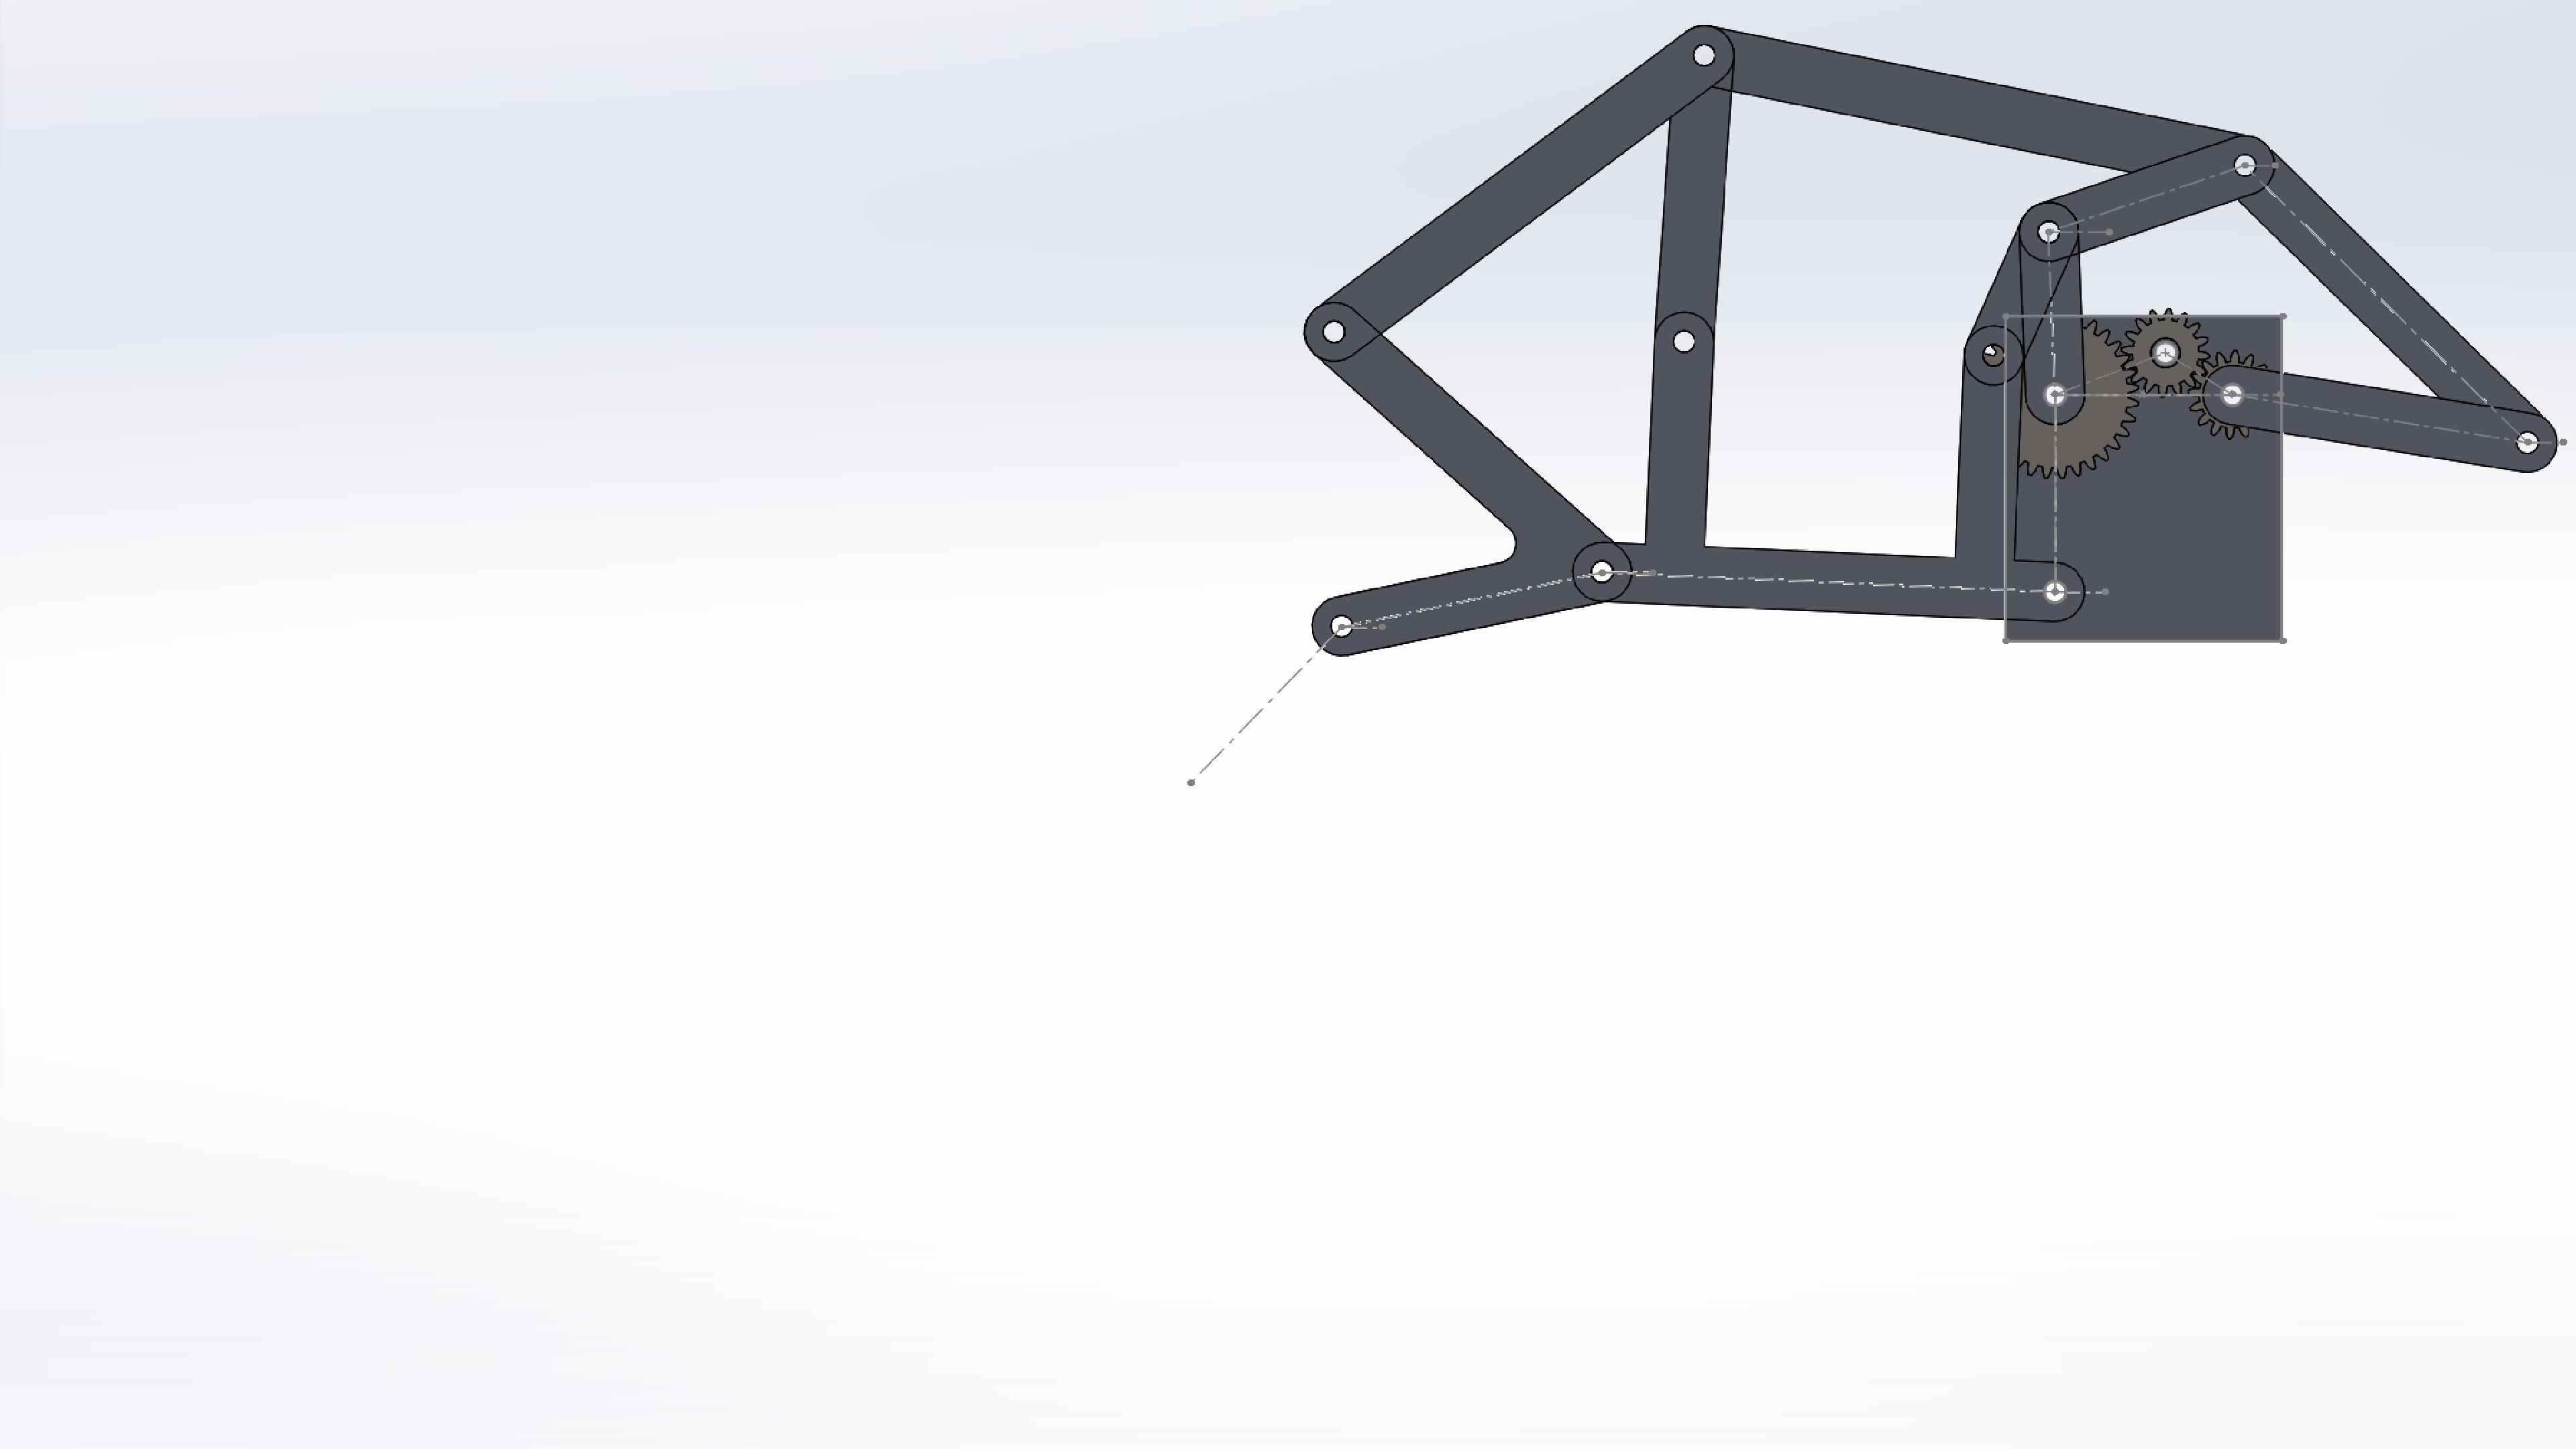
\includegraphics[width=\columnwidth,trim=330bp 195bp 0bp 0bp,clip]{CAD_semilla12.png}
\caption{CAD model of the mechanism optimized with DE, seed 12, used in the motion study.}
\label{fig:cad}
\end{figure}

The error between two corresponding trajectories is calculated as
\begin{equation}
\mathrm{RMSE}=\sqrt{\frac{1}{N}\sum_{i=1}^{N}\|\mathbf p_i^{(1)}-\mathbf p_i^{(2)}\|^2}.
\end{equation}
Table~\ref{tab:simulacion} distinguishes the CAD--model error from the error with respect to the target. The maximum CAD--model differences are 0.1150 mm at PIP and 0.2214 mm at DIP. This comparison verifies that the assembly reproduces the calculated kinematics; it does not constitute a measurement of a physical prototype.

\begin{table}[t]
\caption{Position RMSE of the DE mechanism from seed 12}
\label{tab:simulacion}\centering\footnotesize
\begin{tabular}{lrr}\toprule Comparison & PIP (mm) & DIP (mm)\\\midrule
SolidWorks--model (60)&0.1065&0.1124\\
SolidWorks--target (59)&0.2448&0.3884\\
Model--target (59)&0.2178&0.3618\\\bottomrule
\end{tabular}
\end{table}

\section{Discussion}
The selected mechanism maintains assembly throughout the simulated motion. DE constructs each new solution from differences between individuals; the real-coded GA combines selection, SBX crossover, and polynomial mutation. Both methods find mechanisms that follow the reference, although their solutions are not identical.

For this application, the choice depends on the design priority. If the lowest trajectory error among the selected solutions is sought, GA offers the best result. If a lower sum of lengths and lower calculated height over the finger are sought, DE is preferable. For this reason, the DE solution is taken to CAD, without ruling out GA as an alternative. The smaller size may help reduce volume over the hand, but weight and comfort must be verified with the physical design.

To review the influence of the weights, $J$ is recalculated for the same designs by multiplying the angular residuals by 0.5, 1, and 2, without changing the penalties. Since the residuals are squared, their contribution to $J$ is multiplied by 0.25, 1, and 4. The DE/GA means are, respectively, 0.000496/0.000543, 0.001484/0.001504, and 0.005437/0.005352 mm$^2$. The ordering changes in the last case: the comparison depends on how much angular tracking is valued. The optimization is not repeated, and dimensions or trajectories are not modified.

The study is limited to the available angular reference and the indicated measurements. The lack of identification of the original record prevents confirmation that the motion corresponds to a precision pinch; the results demonstrate tracking of that reference and CAD--model correspondence, not validation of the grasp type. The simulation also does not assess loads, manufacturing clearances, or interference between solids. These checks are necessary before using the mechanism on a person.

\section{Conclusion}
Partial dimensional synthesis of a finger exoskeleton mechanism is obtained through DE and GA under the same formulation, objective function, and evaluation budget, with 20 seeds per method. The selected GA solution obtains lower global trajectory error: 0.198 mm versus 0.298 mm for DE. DE delivers a lower sum of lengths: 328.29 mm versus 353.36 mm, so it is selected to continue the development of a compact mechanism.

The SolidWorks assembly from seed 12 reproduces the model trajectories with RMSEs of 0.106 mm at PIP and 0.112 mm at DIP. The kinematic correspondence between both is confirmed. Future work includes extending the analysis to the complete three-phalanx mechanism and checking motion through a prototype and trajectory measurements.

\ifdefined\versionciega
  \IEEEtriggeratref{2}
\fi
\begin{thebibliography}{18}
\bibitem{r1} N. J. Jarque-Bou, M. Atzori, and H. Müller, ``A large calibrated database of hand movements and grasps kinematics,'' \emph{Scientific Data}, vol. 7, art. 12, 2020, doi: \doi{10.1038/s41597-019-0349-2}.
\bibitem{r2} K. Xia \emph{et al.}, ``Hand exoskeleton design and human--machine interaction strategies for rehabilitation,'' \emph{Bioengineering}, vol. 9, no. 11, art. 682, 2022, doi: 10.3390/bioengineering9110682.
\bibitem{r3} R. John Varghese, G. Mukherjee, and A. Deshpande, ``Designing physical human-robot interaction interfaces: A scalable method for simulation based design,'' \emph{Frontiers in Neurorobotics}, vol. 15, art. 727534, 2022, doi: \doi{10.3389/fnbot.2021.727534}.
\bibitem{r4} J. A. Cabrera, A. Simon, and M. Prado, ``Optimal synthesis of mechanisms with genetic algorithms,'' \emph{Mechanism and Machine Theory}, vol. 37, no. 10, pp. 1165--1177, 2002, doi: 10.1016/S0094-114X(02)00051-4.
\bibitem{r5} S. Sleesongsom and S. Bureerat, ``Four-bar linkage path generation through self-adaptive population size teaching-learning based optimization,'' \emph{Knowledge-Based Systems}, vol. 135, pp. 180--191, 2017, doi: \doi{10.1016/j.knosys.2017.08.012}.
\bibitem{r6} V. Kachitvichyanukul, ``Comparison of three evolutionary algorithms: GA, PSO, and DE,'' \emph{Industrial Engineering \& Management Systems}, vol. 11, no. 3, pp. 215--223, 2012, doi: 10.7232/iems.2012.11.3.215.
\bibitem{r7} T. Tušar and B. Filipič, ``Differential evolution versus genetic algorithms in multiobjective optimization,'' in \emph{Evolutionary Multi-Criterion Optimization}, LNCS 4403, 2007, pp. 257--271, doi: 10.1007/978-3-540-70928-2\_22.
\bibitem{r8} S. M. Varedi-Koulaei, M. Mohammadi, M. A. M. Mohammadi, and M. Bamdad, ``Optimal synthesis of the Stephenson-II linkage for finger exoskeleton using swarm-based optimization algorithms,'' \emph{Journal of Bionic Engineering}, vol. 20, no. 4, pp. 1569--1584, 2023, doi: \doi{10.1007/s42235-022-00327-5}.
\bibitem{r9} Bilal, M. Pant, H. Zaheer, L. Garcia-Hernandez, and A. Abraham, ``Differential evolution: A review of more than two decades of research,'' \emph{Engineering Applications of Artificial Intelligence}, vol. 90, art. 103479, 2020, doi: \doi{10.1016/j.engappai.2020.103479}.
\bibitem{r10} A. K. Qin, V. L. Huang, and P. N. Suganthan, ``Differential evolution algorithm with strategy adaptation for global numerical optimization,'' \emph{IEEE Trans. Evolutionary Computation}, vol. 13, no. 2, pp. 398--417, 2009, doi: \doi{10.1109/TEVC.2008.927706}.
\bibitem{r17} J. A. Caballero-Mora \emph{et al.}, ``UR3 collaborative robot inverse kinematics using metaheuristic optimization: A unified comparative and experimental evaluation,'' \emph{Applied System Innovation}, vol. 9, no. 7, art. 140, 2026, doi: 10.3390/asi9070140.
\bibitem{r13} T. Akiba, S. Sano, T. Yanase, T. Ohta, and M. Koyama, ``Optuna: A next-generation hyperparameter optimization framework,'' in \emph{Proc. ACM SIGKDD}, 2019, pp. 2623--2631, doi: \doi{10.1145/3292500.3330701}.
\bibitem{r14} S. Das, S. S. Mullick, and P. N. Suganthan, ``Recent advances in differential evolution -- An updated survey,'' \emph{Swarm and Evolutionary Computation}, vol. 27, pp. 1--30, 2016, doi: \doi{10.1016/j.swevo.2016.01.004}.
\bibitem{r15} S. Chakraborty, A. K. Saha, A. E. Ezugwu, J. O. Agushaka, R. A. Zitar, and L. Abualigah, ``Differential evolution and its applications in image processing problems: A comprehensive review,'' \emph{Archives of Computational Methods in Engineering}, vol. 30, no. 2, pp. 985--1040, 2023, doi: \doi{10.1007/s11831-022-09825-5}.
\bibitem{r16} K. Deb and R. B. Agrawal, ``Simulated binary crossover for continuous search space,'' \emph{Complex Systems}, vol. 9, no. 2, pp. 115--148, 1995.
\bibitem{rwilcoxon} F. Wilcoxon, ``Individual comparisons by ranking methods,'' \emph{Biometrics Bulletin}, vol. 1, no. 6, pp. 80--83, 1945, doi: \doi{10.2307/3001968}.
\bibitem{r11} H. G. Barrow, J. M. Tenenbaum, R. C. Bolles, and H. C. Wolf, ``Parametric correspondence and chamfer matching: Two new techniques for image matching,'' in \emph{Proc. IJCAI}, 1977, pp. 659--663.
\bibitem{r12} J. C. Gower, ``Generalized Procrustes analysis,'' \emph{Psychometrika}, vol. 40, no. 1, pp. 33--51, 1975, doi: \doi{10.1007/BF02291478}.
\end{thebibliography}

\end{document}